\chapter{推前测度}
\label{chap:pushforward-measures}

在$[-1,1]$上均匀地撒一把质量，再把每一点$x$送到$x^2$。落到$[0,1]$中某个区间里的质量有多少？对$[0,1]$上的函数积分时，能否回到原来的区间上计算？这类问题在坐标变换、取部分坐标和随机变量的函数中反复出现。它们的共同结构是：原空间上有一个测度，一个可测映射把点送到目标空间，我们要描述目标空间上的质量分布，并在两个空间之间改写积分。

本章分三步回答。第一节用集合的原像定义目标空间的测度，即推前测度，核对它是测度并且与映射的复合相容，再用有限集合与坐标投影的例子观察质量怎样转移、汇合，以及哪些信息被保留。第二节证明推前积分恒等式：目标空间上的积分等于原空间上复合函数的积分。这一恒等式只用到原像，不要求映射可逆，也不要求任何密度。

第三节在目标空间选定参考测度，讨论推前测度何时有密度、密度怎样计算。这一步把推前与上一章的换测度结合起来，分三种机制处理：欧氏开集之间的光滑可逆映射靠逆映射的Jacobian因子，分成有限个可逆光滑分支的映射要对落到同一点的各分支求和，坐标投影则对舍去的坐标积分。常值映射的例子说明，推前测度相对于Lebesgue测度的密度未必存在。

本章所用的可测映射、测度延拓的唯一性来自第~\ref{chap:measure}章，单调收敛定理与Tonelli、Fubini定理来自第~\ref{chap:integration}章，相对密度与换测度公式来自第~\ref{chap:measure-densities}章。曲面上的面积测度、一般非线性降维所需的沿纤维积分超出本章范围；流形上的体积与积分在第~\ref{chap:manifold-calculus}章研究。

\section{推前测度的构造}
\label{sec:push-construction}

可测映射保证目标空间中的集合问题在原空间有意义：目标可测集的原像仍然可测。若原空间还配有测度，就可以回答“映射的输出落在$B$中的质量有多少”：把会被送进$B$的点全部找出来，累计它们的质量。本节用这一想法定义推前测度，核对它的可数可加性与复合规则，再用例子观察不同映射怎样改变质量的分配。积分与密度的计算放在后两节。

\subsection{推前测度的定义}
\label{sec:push-definition}

设$(X,\mathcal A)$与$(Y,\mathcal B)$是可测空间，$T:X\to Y$可测，$\mu$是$(X,\mathcal A)$上的测度。对$B\in\mathcal B$，输出落在$B$中的点恰好组成原像$T^{-1}(B)=\{x\in X:T(x)\in B\}$，它属于$\mathcal A$，于是可以取它的质量作为$B$的质量。

\begin{definition}[推前测度]
\label{def:push-pushforward}
在上述记号下，令
\[
(T_\#\mu)(B)=\mu\bigl(T^{-1}(B)\bigr),\qquad B\in\mathcal B ,
\]
称$T_\#\mu$为$\mu$在$T$下的\term{推前测度}（pushforward measure）。
\end{definition}

定义只用原像，所以先要核对$T_\#\mu$确实是测度。空集的原像是空集，故$(T_\#\mu)(\varnothing)=0$。设$B_1,B_2,\ldots\in\mathcal B$两两不交，则它们的原像也两两不交：一个$x$若同时属于$T^{-1}(B_n)$与$T^{-1}(B_m)$，$T(x)$就同时属于$B_n$与$B_m$。原像保持并运算，$T^{-1}(\bigcup_nB_n)=\bigcup_nT^{-1}(B_n)$，由$\mu$的可数可加性，
\[
(T_\#\mu)\Bigl(\bigcup_nB_n\Bigr)=\mu\Bigl(\bigcup_nT^{-1}(B_n)\Bigr)=\sum_n\mu\bigl(T^{-1}(B_n)\bigr)=\sum_n(T_\#\mu)(B_n).
\]
所以$T_\#\mu$是$(Y,\mathcal B)$上的测度。又$T^{-1}(Y)=X$，总质量不变：$(T_\#\mu)(Y)=\mu(X)$。特别地，有限测度推前后仍有限，概率测度推前后仍是概率测度。

\paragraph{复合规则}
复杂的映射常常可以拆成几步简单的映射。设$S:(Y,\mathcal B)\to(Z,\mathcal C)$也可测，复合$S\circ T$可测，并且原像按逆序作用：$(S\circ T)^{-1}(C)=T^{-1}(S^{-1}(C))$。于是对$C\in\mathcal C$，
\[
\bigl((S\circ T)_\#\mu\bigr)(C)=\mu\bigl(T^{-1}(S^{-1}(C))\bigr)=(T_\#\mu)\bigl(S^{-1}(C)\bigr)=\bigl(S_\#(T_\#\mu)\bigr)(C),
\]
即$(S\circ T)_\#\mu=S_\#(T_\#\mu)$。分两步传递质量与一步传递质量的结果相同，所以可以把映射拆开逐步计算推前。

\paragraph{总质量保持，$\sigma$有限性未必保持}
总质量不变，但$\sigma$有限性可能丢失，因为推前可以把无限多份有限质量集中到一点。在$\mathbb N$上取计数测度$\mu$，它是$\sigma$有限的。令$T$把$\mathbb N$映到单点集$Y=\{y\}$，则$(T_\#\mu)(\{y\})=\mu(\mathbb N)=+\infty$；$Y$的可测子集只有$\varnothing$与$\{y\}$，无法写成有限质量集合的可数并。后面需要测度延拓的唯一性或Radon–Nikodym定理时，推前测度的$\sigma$有限性必须单独核对。

\subsection{映射下的质量转移}
\label{sec:push-mass-transfer}

定义只说明了怎样计算，下面用例子看推前测度到底记录了什么。我们先按原像确定目标测度，不预设它有任何密度。

\paragraph{一一映射与多对一映射}
若$T$是一一映射，每个输出点只收到一个原像的质量，推前只是把质量换了位置。设$X=\{1,2,3,4\}$上的测度$\mu$给四个点分别赋权$0.1,0.2,0.3,0.4$，$T$把$k$送到$Y=\{a,b,c,d\}$中的第$k$个点，则$T_\#\mu$给$a,b,c,d$的权重仍是$0.1,0.2,0.3,0.4$。

推前不要求$T$是单射。若几个点被送到同一个输出，它们的质量在输出处相加。仍取上面的$\mu$，令$T(1)=T(3)=a$，$T(2)=T(4)=b$，则$T^{-1}(\{a\})=\{1,3\}$，$T^{-1}(\{b\})=\{2,4\}$，所以
\[
T_\#\mu=0.4\,\delta_a+0.6\,\delta_b .
\]
原来的四个点在输出端只剩两个，总量仍为$1$，见图~\ref{fig:push-merge}(a)。从$T_\#\mu$出发已经无法分辨$a$处的$0.4$来自哪两个点，汇合丢掉了原像之间的区分。

推前还可以把连续分布的质量汇合成点质量。令$\mu=\lambda|_{[0,1]}$，$T(x)=\lfloor2x\rfloor$。$[0,1]$中的原像分别是$T^{-1}(\{0\})\cap[0,1]=[0,\tfrac12)$，$T^{-1}(\{1\})\cap[0,1]=[\tfrac12,1)$，$T^{-1}(\{2\})\cap[0,1]=\{1\}$，所以$T_\#\mu=\tfrac12\delta_0+\tfrac12\delta_1$。每个单点在$\mu$下质量为零，推前后却出现了质量$\tfrac12$的点，因为原像不是单点，而是一段区间。

\begin{figure}[!htbp]
  \centering
  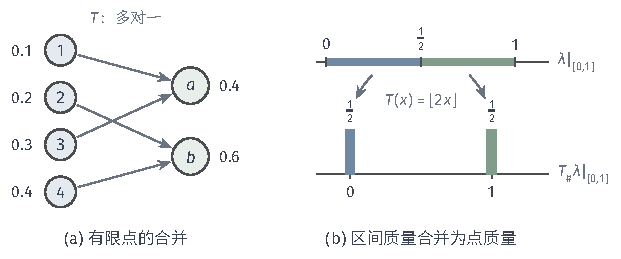
\includegraphics[width=105.1mm]{figures/02-abstract-mathematics/01-metric-and-measure/tikz/c2-pushforward-merge/figure.pdf}
  \caption{推前测度累计原像的质量。(a)四个带权点经多对一映射送到$a,b$两点，$a$收集点$1,3$的权重$0.1+0.3=0.4$，$b$收集点$2,4$的权重$0.2+0.4=0.6$；(b)$[0,1]$上的长度测度经$T(x)=\lfloor2x\rfloor$推前，原像$[0,\tfrac12)$与$[\tfrac12,1)$的长度分别汇集为点$0$和点$1$处的质量$\tfrac12$，单点$\{1\}$的长度为零，不贡献质量。}
  \label{fig:push-merge}
\end{figure}

\paragraph{平移与伸缩}
在实轴上，平移$T(x)=x+t$满足$T^{-1}(B)=B-t$，由Lebesgue测度的平移不变性，$T_\#\lambda=\lambda$；这种使$T_\#\mu=\mu$的映射称为\term{保持测度}（measure-preserving）的映射。伸缩则改变长度。令$T(x)=2x$，区间$(a,b]$的原像是$(a/2,b/2]$，所以$(T_\#\lambda)((a,b])=(b-a)/2$。两个测度$T_\#\lambda$与$\tfrac12\lambda$在全部半开区间上一致，并在每个$(-n,n]$上有限，由测度延拓的唯一性，$T_\#\lambda=\tfrac12\lambda$。把实轴拉长一倍，同一个输出区间只收集到原来一半长度的输入。这个例子将在第~\ref{sec:push-smooth-change}小节用来核对坐标换元中因子的方向。

\paragraph{坐标投影}
多元问题中最常见的多对一映射是坐标投影。设$\mu$是$\mathcal B(\mathbb R^d)$上的测度，$1\leq k<d$，$\pi(\bm x)=(x_1,\ldots,x_k)$。$\pi$连续，因而Borel可测，且对$B\in\mathcal B(\mathbb R^k)$有$\pi^{-1}(B)=B\times\mathbb R^{d-k}$，所以
\[
(\pi_\#\mu)(B)=\mu\bigl(B\times\mathbb R^{d-k}\bigr).
\]
$\pi_\#\mu$称为$\mu$在前$k$个坐标上的\term{边缘测度}（marginal measure）。它只回答形如“前$k$个坐标落在$B$中”的问题，保留的是$\mu$在柱形集合$B\times\mathbb R^{d-k}$上的值；后$d-k$个坐标怎样分布、两组坐标之间怎样关联，都不再能从边缘测度读出。概率论中由联合分布得到边缘分布正是这一操作，可参考\BookChapterRef{chap:random-vectors}{卷七“随机向量与联合分布”章}。

\begin{example}[点质量与单位正方形的投影]
\label{ex:push-projection}
在$\mathbb R^2$上取$\mu=0.2\,\delta_{(0,0)}+0.3\,\delta_{(0,1)}+0.5\,\delta_{(1,1)}$。第一坐标的投影$\pi_1$把$(0,0)$与$(0,1)$都送到$0$，所以$(\pi_1)_\#\mu=0.5\,\delta_0+0.5\,\delta_1$；第二坐标的投影把$(0,1)$与$(1,1)$都送到$1$，所以$(\pi_2)_\#\mu=0.2\,\delta_0+0.8\,\delta_1$。两个边缘测度合起来也不能恢复$\mu$：四个格点上的质量只要横向与纵向的合计相同，边缘就相同。例如$0.1\,\delta_{(0,0)}+0.1\,\delta_{(1,0)}+0.4\,\delta_{(0,1)}+0.4\,\delta_{(1,1)}$的两个边缘也是$0.5\,\delta_0+0.5\,\delta_1$与$0.2\,\delta_0+0.8\,\delta_1$，它却给$(1,0)$正质量。

再取$\nu=\lambda_2|_{[0,1]^2}$。对$B=(a,b]$，$\pi_1^{-1}(B)\cap[0,1]^2=((a,b]\cap[0,1])\times[0,1]$是一个矩形，面积等于$\lambda((a,b]\cap[0,1])$。于是$(\pi_1)_\#\nu$与$\lambda|_{[0,1]}$在全部半开区间上一致，总量都为$1$，由延拓的唯一性，二者相等。图~\ref{fig:push-projection}画出了两种情形。
\end{example}

\begin{figure}[!htbp]
  \centering
  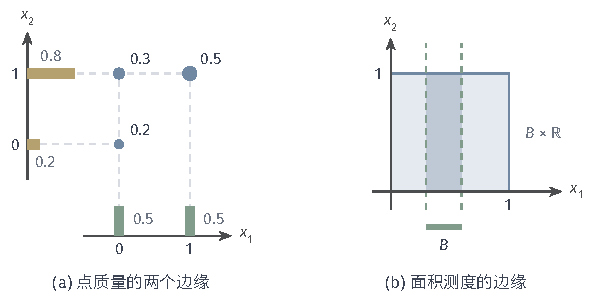
\includegraphics[width=100.9mm]{figures/02-abstract-mathematics/01-metric-and-measure/tikz/c2-projection-marginal/figure.pdf}
  \caption{坐标投影产生的边缘测度。(a)平面上三个点质量$0.2,0.3,0.5$，向横轴投影得到$0.5\delta_0+0.5\delta_1$，向纵轴投影得到$0.2\delta_0+0.8\delta_1$；(b)单位正方形上的面积测度，横轴区间$B$的边缘质量等于竖条$B\times\mathbb R$与正方形之交的面积，结果是$[0,1]$上的长度。}
  \label{fig:push-projection}
\end{figure}

边缘测度的总量与原测度相同，但$\sigma$有限性同样可能丢失：对整个平面上的$\lambda_2$，任一非退化区间$B$都有$(\pi_1)_\#\lambda_2(B)=\lambda_2(B\times\mathbb R)=+\infty$。上面的点质量例子还说明，输出测度不一定有密度，它可以是离散的。推前测度上的积分怎样计算，是下一节的问题；边缘测度何时有密度、怎样由原测度的密度算出，在第~\ref{sec:push-projection-density}小节处理。

\section{推前积分恒等式}
\label{sec:push-integral-identity}

上一节确定了目标空间上的质量。现在对目标空间上的函数$g$积分：$\int_Yg\,\mathrm d(T_\#\mu)$能否回到原空间计算？直观上，每个点$x$带着质量被送到$T(x)$，在那里读取函数值$g(T(x))$，所以应当有$\int_Yg\,\mathrm d(T_\#\mu)=\int_Xg\circ T\,\mathrm d\mu$。先对指示函数核对。若$g=\mathbf 1_B$，左端是$(T_\#\mu)(B)=\mu(T^{-1}(B))$；而$\mathbf 1_B(T(x))=1$当且仅当$x\in T^{-1}(B)$，即$\mathbf 1_B\circ T=\mathbf 1_{T^{-1}(B)}$，右端也等于$\mu(T^{-1}(B))$。沿积分的构造步骤推广，就得到一般结论。

\begin{theorem}[推前积分恒等式]
\label{thm:push-integral-identity}
设$(X,\mathcal A,\mu)$是测度空间，$T:(X,\mathcal A)\to(Y,\mathcal B)$可测。
\begin{enumerate}
\item 对每个可测$g:Y\to[0,+\infty]$，
\begin{equation}
\int_Yg\,\mathrm d(T_\#\mu)=\int_Xg\circ T\,\mathrm d\mu ,
\label{eq:push-integral-identity}
\end{equation}
两边可以同为$+\infty$。
\item 对可测的实值或复值$g$，$g$关于$T_\#\mu$可积当且仅当$g\circ T$关于$\mu$可积，此时式~\eqref{eq:push-integral-identity}成立且两边有限。
\end{enumerate}
\end{theorem}

\begin{proof}
$g\circ T$是可测映射的复合，因而可测。(1) 指示函数的情形已在上面核对。对非负简单函数$s=\sum_ic_i\mathbf 1_{B_i}$，$s\circ T=\sum_ic_i\mathbf 1_{B_i}\circ T$，两边由线性性相等。对一般非负可测$g$，取非负简单函数$s_n\uparrow g$，则$s_n\circ T\uparrow g\circ T$，两边分别用单调收敛定理取极限。

(2) 由$\lvert g\circ T\rvert=\lvert g\rvert\circ T$，把(1)用于$\lvert g\rvert$，两边的绝对积分相等，可积性等价。实值时$(g\circ T)^\pm=g^\pm\circ T$，对正部和负部分别用(1)后相减，两边都是有限数之差；复值时对实部和虚部分别处理。
\end{proof}

定理只用到可测性与推前测度的定义。它不要求$T$可逆或可微，不要求$X,Y$有距离或坐标，也不要求$T_\#\mu$相对于任何参考测度有密度。这里沿映射转移的是测度，被积函数相应地复合上$T$；这与上一章的换测度公式不同，那里点不移动，被积函数不变，只是累计权重乘上密度。

恒等式可以从两个方向读。已知$\mu$时，它把目标空间上的积分化为原空间上的积分，例如随机变量的函数的期望，可以直接在原来的概率空间上计算，不必先求出输出的分布。反过来，它说明对复合函数$g\circ T$的累计只取决于$T$把质量送到了哪里：两个映射若推前出同一个测度，所有形如$\int g\circ T\,\mathrm d\mu$的积分都相同。

\begin{example}[有限集合上的分组汇总]
\label{ex:push-finite-sum}
取$X=\{1,2,3,4\}$，$\mu(\{k\})=k/10$；$Y=\{0,1\}$，$T(1)=T(3)=1$，$T(2)=T(4)=0$。输出点$0$的原像是$\{2,4\}$，所以$(T_\#\mu)(\{0\})=0.2+0.4=0.6$；同理$(T_\#\mu)(\{1\})=0.1+0.3=0.4$。取$g(0)=5$、$g(1)=2$，左端是$5\times0.6+2\times0.4=3.8$；右端逐个原像点计算$g(T(k))\mu(\{k\})$，得$2\times0.1+5\times0.2+2\times0.3+5\times0.4=3.8$。
\end{example}

图~\ref{fig:push-finite-sum}显示了两种算法的差别：右端逐点累计，左端先把映到同一输出点的质量合并，再乘以该点的函数值。整个计算没有用到任何“输出密度”，输出测度本身就是两个原子。

\begin{figure}[!htbp]
\centering
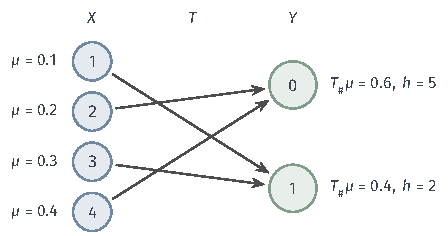
\includegraphics[width=75.812mm]{figures/02-abstract-mathematics/01-metric-and-measure/tikz/c3-pushforward-change/figure.pdf}
\caption{有限集合上的推前与换元。输入点$k=1,2,3,4$的质量为$k/10$，映射$T$把$2,4$送到$0$、把$1,3$送到$1$，输出质量分别为$0.6$与$0.4$。取$h(0)=5$、$h(1)=2$（正文记作$g$），按输出点汇总与按输入点逐个累计都得到$3.8$。}
\label{fig:push-finite-sum}
\end{figure}

\paragraph{连续情形与复合}
在$[0,1]$上取$\mu=\lambda|_{[0,1]}$，$T(x)=\lfloor2x\rfloor$，上一节已求出$T_\#\mu=\tfrac12\delta_0+\tfrac12\delta_1$。对$g(y)=y^2+1$，左端$\tfrac12g(0)+\tfrac12g(1)=\tfrac12+1=\tfrac32$；右端$\int_0^1(\lfloor2x\rfloor^2+1)\,\mathrm dx=\int_0^{1/2}1\,\mathrm dx+\int_{1/2}^12\,\mathrm dx=\tfrac32$，单点$x=1$不影响积分。若接着再作映射$S:Y\to Z$，由$(S\circ T)_\#\mu=S_\#(T_\#\mu)$，式~\eqref{eq:push-integral-identity}可以逐级使用：$\int_Zk\,\mathrm d((S\circ T)_\#\mu)=\int_Yk\circ S\,\mathrm d(T_\#\mu)=\int_Xk\circ S\circ T\,\mathrm d\mu$。

\paragraph{可积性条件}
第2条中的可积性条件不能省。在$(0,1)$上取$\mu=\lambda|_{(0,1)}$，$T(x)=1/x$，把质量送到$(1,\infty)$。对$g(y)=\sin y$，$\int_{(0,1)}\lvert\sin(1/x)\rvert\,\mathrm dx\leq1$，两边都可积，恒等式成立。对$g(y)=y$，$\int_0^1(1/x)\,\mathrm dx=+\infty$，按第1条两边同为$+\infty$，仍是一个正确的等式；但若换成带符号的$g(y)=y\sin y$，可以验证两边的正部与负部积分都是$+\infty$，这时式~\eqref{eq:push-integral-identity}没有意义，而不是不成立。实际使用时，应先对$\lvert g\rvert$用第1条确认可积，再写出有符号的等式。

\section{映射后的密度}
\label{sec:push-mapped-densities}

推前积分恒等式把目标空间上的积分送回原空间。但在目标空间上直接计算时，我们往往希望把推前测度写成一个熟悉的参考测度的加权形式，就像在实轴上用概率密度代替分布本身。

设在目标空间$Y$上选定参考测度$\lambda$，并假设推前测度有密度
\[
h=\frac{\mathrm d(T_\#\mu)}{\mathrm d\lambda}.
\]
对非负可测$g$，连续使用推前积分恒等式与第~\ref{chap:measure-densities}章的换测度公式，得到两步改写
\begin{equation}
\int_Xg\circ T\,\mathrm d\mu=\int_Yg\,\mathrm d(T_\#\mu)=\int_Ygh\,\mathrm d\lambda .
\label{eq:push-two-step}
\end{equation}

第一步沿映射转移测度并复合被积函数，第二步留在$Y$上，只把累计权重换成$h$。两步依据不同的定理，条件也不同：第一步对任何可测映射成立，第二步要求密度存在。

\paragraph{密度未必存在}
密度存在的必要条件是$T_\#\mu\ll\lambda$，即对每个$\lambda$零测集$N\subset Y$，都有
\[
\mu\bigl(T^{-1}(N)\bigr)=0 .
\]
也就是说，映射不能把正的质量压进目标空间的零测集。

常值映射给出最简单的反例。令$X=[0,1]$，$\mu=\lambda|_{[0,1]}$，$T(x)=c$。当$c\in B$时$T^{-1}(B)=[0,1]$，否则$T^{-1}(B)=\varnothing$，所以
\[
T_\#\mu=\delta_c .
\]
单点$\{c\}$是Lebesgue零测集，却承载全部质量，$T_\#\mu$与$\lambda$相互奇异，没有Lebesgue密度。映射把一段区间压成一点，原像$T^{-1}(\{c\})$有正长度，这就是失败的原因。

所以计算映射后的密度，要先确认映射不把正质量压进零测集。下面三个小节分别处理三种常见结构：光滑可逆映射、分成有限个可逆光滑分支的映射，以及坐标投影。

\subsection{光滑坐标换元}
\label{sec:push-smooth-change}

设$U,V\subset\mathbb R^d$是开集。若$T:U\to V$是双射，$T$与$T^{-1}$都连续可微，就称$T$为$C^1$\term{微分同胚}（diffeomorphism）。对$T^{-1}\circ T=\mathrm{id}$求导，得
\[
DT^{-1}\bigl(T(\bm x)\bigr)\,DT(\bm x)=\bm I .
\]

取行列式可知\term{Jacobian行列式}（Jacobian determinant）$\det DT(\bm x)$处处不为零，并且
\begin{equation}
\bigl\lvert\det DT^{-1}(\bm y)\bigr\rvert=\frac{1}{\bigl\lvert\det DT\bigl(T^{-1}(\bm y)\bigr)\bigr\rvert},\qquad\bm y\in V .
\label{eq:push-inverse-jacobian}
\end{equation}
本小节记$S=T^{-1}:V\to U$，它也是$C^1$微分同胚。所有函数与集合都取Borel可测的版本。

\paragraph{Lebesgue测度的推前}
先以$\lambda_d|_U$为原测度，问它推前到$V$上是什么。由定义，小盒子$Q\subset V$得到的质量是它的原像$S(Q)$的体积。$S$在小盒子上近似于线性映射$DS(\bm y)$，线性映射把体积乘以行列式的绝对值，所以
\[
(T_\#\lambda_d)(Q)=\lambda_d\bigl(S(Q)\bigr)\approx\bigl\lvert\det DS(\bm y)\bigr\rvert\,\lambda_d(Q).
\]
这说明推前测度的密度应当是逆映射的Jacobian因子。

用极坐标算一个具体的小盒子。取$S(r,\theta)=(r\cos\theta,r\sin\theta)$，$T$是它的逆，Jacobian行列式为
\[
\det DS(r,\theta)=r .
\]
取$Q=[1,1.2]\times[0.3,0.8]$，它的面积是$0.2\times0.5=0.1$。它的原像$S(Q)$是一块环形扇区，面积是
\[
\lambda_2\bigl(S(Q)\bigr)=\int_{0.3}^{0.8}\int_1^{1.2}r\,\mathrm dr\,\mathrm d\theta=0.5\times\frac{1.2^2-1^2}{2}=0.11 .
\]

两个面积之比是$0.11/0.1=1.1$，恰好是$Q$中心$r=1.1$处的$\lvert\det DS\rvert$。图~\ref{fig:push-local-volume}画出了这个小盒子和它的原像。绿色虚线是线性化$DS$给出的平行四边形，面积也是$1.1\times0.1=0.11$；它与真实的环形扇区只差一些边角，盒子越小差得越少。

\begin{BookInlineFigure}
  \centering
  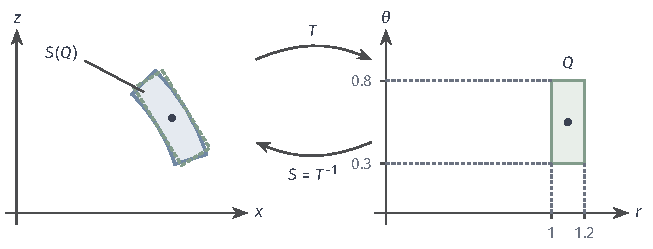
\includegraphics[width=110.539mm]{figures/04-spaces-measures-and-geometry/02-measure/tikz/push-local-volume/figure.pdf}
  \caption{小盒子的原像决定局部密度。右图是极坐标平面上的盒子$Q=[1,1.2]\times[0.3,0.8]$，左图蓝色区域是它在$(x,z)$平面的原像$S(Q)$，绿色虚线是中心处线性化$DS$给出的平行四边形，黑点是中心。两张图用相同的比例尺，面积分别为$0.1$与$0.11$，比值$1.1$等于$\lvert\det DS\rvert$在中心的值。}
  \label{fig:push-local-volume}
\end{BookInlineFigure}

把这个局部比例严格化，需要卷二的经典换元公式。设$E\subset V$是紧Jordan区域，$S(E)$也是Jordan区域，$f$在$S(E)$上连续，则
\begin{equation}
\int_{S(E)}f(\bm x)\,\mathrm d\bm x=\int_Ef\bigl(S(\bm y)\bigr)\,\lvert\det DS(\bm y)\rvert\,\mathrm d\bm y .
\label{eq:push-classical-change}
\end{equation}
公式的陈述和证明思路见\BookChapterRef{chap:region-integrals}{卷二第24章“区域积分”}。证明需要对细分作一致的误差控制，篇幅较长，读者可查阅实分析教材。我们只用它在闭盒子上、$f\equiv1$时的情形，再用测度延拓的唯一性推广到一切Borel集。

\begin{theorem}[微分同胚下Lebesgue测度的推前]
\label{thm:push-lebesgue-diffeo}
设$T:U\to V$是$C^1$微分同胚。则对每个Borel集$B\subset V$，
\begin{equation}
(T_\#\lambda_d)(B)=\lambda_d\bigl(T^{-1}(B)\bigr)=\int_B\bigl\lvert\det DT^{-1}(\bm y)\bigr\rvert\,\mathrm d\bm y ,
\label{eq:push-lebesgue-diffeo}
\end{equation}
即$T_\#(\lambda_d|_U)$相对于$\lambda_d|_V$的密度是$\lvert\det DT^{-1}\rvert$。
\end{theorem}

\begin{proof}
令$\nu(B)=\int_B\lvert\det DS\rvert\,\mathrm d\bm y$，它是$V$的Borel集上的测度。证明分两步：先在闭盒子上比较$T_\#\lambda_d$与$\nu$，再推广到全部Borel集。

设$Q\subset V$是闭盒子，允许退化。$S$是同胚，所以$S(Q)$是紧集，边界是$S(\partial Q)$。$S$在凸紧集$Q$上连续可微，由中值不等式在$Q$上Lipschitz，因而把$Q$中容量为零的集合映成容量为零的集合。$\partial Q$的容量为零，所以$S(\partial Q)$的容量为零，$S(Q)$是紧Jordan区域。

对$E=Q$、$f\equiv1$用式~\eqref{eq:push-classical-change}。Jordan区域上连续函数的Riemann积分等于Lebesgue积分，于是
\[
(T_\#\lambda_d)(Q)=\lambda_d\bigl(S(Q)\bigr)=\int_Q\lvert\det DS(\bm y)\rvert\,\mathrm d\bm y=\nu(Q).
\]

含于$V$的闭盒子连同空集对有限交封闭，构成$\pi$系统。$V$的每个开子集都是可数个含于其中的有理端点闭盒子之并，所以这些盒子生成$V$上的Borel $\sigma$代数，并有可数个覆盖$V$。两个测度在每个闭盒子上都有限，因为$S(Q)$紧、$\lvert\det DS\rvert$在$Q$上有界。由第~\ref{chap:measure}章的延拓唯一性，$T_\#\lambda_d=\nu$在$V$的全部Borel集上成立。
\end{proof}

定理说明，推前测度的密度在新坐标$\bm y$处取值，因子是逆映射的Jacobian。由式~\eqref{eq:push-inverse-jacobian}，它也可以写成$1/\lvert\det DT(S(\bm y))\rvert$：$T$在原像附近把体积拉伸的地方，同样多的质量摊到更大的范围，密度就变小。

\paragraph{原测度有密度的情形}
现在设$U$上的测度$\mu$相对于$\lambda_d$有密度$p$。把推前积分恒等式、换测度公式与上一个定理接起来，就得到推前测度的密度。

\begin{theorem}[微分同胚下的推前密度]
\label{thm:push-density-diffeo}
设$T:U\to V$是$C^1$微分同胚，$U$上的测度$\mu$相对于$\lambda_d$有密度$p$。则$T_\#\mu$相对于$V$上的$\lambda_d$有密度
\begin{equation}
q(\bm y)=p\bigl(T^{-1}(\bm y)\bigr)\,\bigl\lvert\det DT^{-1}(\bm y)\bigr\rvert ,\qquad\bm y\in V .
\label{eq:push-density-diffeo}
\end{equation}
\end{theorem}

\begin{proof}
设$B\subset V$是Borel集。由推前测度和密度的定义，
\[
(T_\#\mu)(B)=\mu\bigl(T^{-1}(B)\bigr)=\int_U\mathbf 1_B\bigl(T(\bm x)\bigr)\,p(\bm x)\,\mathrm d\bm x .
\]

因为$\bm x=S(T(\bm x))$，被积函数可以写成$\psi\circ T$，其中
\[
\psi(\bm y)=\mathbf 1_B(\bm y)\,p\bigl(S(\bm y)\bigr)
\]
是$V$上的非负Borel函数。对$\lambda_d|_U$与$T$用推前积分恒等式，再用定理~\ref{thm:push-lebesgue-diffeo}的密度与换测度公式，得到
\[
\begin{aligned}
\int_U\psi\circ T\,\mathrm d\lambda_d&=\int_V\psi\,\mathrm d(T_\#\lambda_d)\\
&=\int_V\psi(\bm y)\,\lvert\det DS(\bm y)\rvert\,\mathrm d\bm y\\
&=\int_Bp\bigl(S(\bm y)\bigr)\,\lvert\det DS(\bm y)\rvert\,\mathrm d\bm y .
\end{aligned}
\]
这正是$(T_\#\mu)(B)=\int_Bq\,\mathrm d\lambda_d$。
\end{proof}

\paragraph{与通常换元公式对照}
通常的积分换元公式中出现的是正向的Jacobian，这与定理~\ref{thm:push-density-diffeo}的因子方向相反。它也可以由定理~\ref{thm:push-lebesgue-diffeo}得到：把定理用于微分同胚$S:V\to U$，得到$S_\#\lambda_d$的密度是$\lvert\det DS^{-1}\rvert=\lvert\det DT\rvert$。

对非负Borel函数$g$，把$g$写成$(g\circ T)\circ S$，用推前积分恒等式，再用这个密度，得到
\begin{equation}
\begin{aligned}
\int_Vg\,\mathrm d\lambda_d&=\int_V(g\circ T)\circ S\,\mathrm d\lambda_d\\
&=\int_Ug\circ T\,\mathrm d(S_\#\lambda_d)\\
&=\int_Ug\bigl(T(\bm x)\bigr)\,\lvert\det DT(\bm x)\rvert\,\mathrm d\bm x .
\end{aligned}
\label{eq:push-jacobian-change}
\end{equation}

两个公式回答不同的问题。式~\eqref{eq:push-density-diffeo}问的是“新坐标$\bm y$处每单位体积有多少质量”，所以因子在新坐标上取值，是逆映射的Jacobian。式~\eqref{eq:push-jacobian-change}把新坐标上的体积元改写到原坐标上，所以因子在原坐标上取值，是正向映射的Jacobian。

用第~\ref{sec:push-mass-transfer}小节的伸缩$T(x)=2x$核对方向。这时$T^{-1}(y)=y/2$，导数的绝对值是$\tfrac12$，由定理~\ref{thm:push-lebesgue-diffeo}，
\[
T_\#\lambda=\tfrac12\lambda ,
\]
与按原像直接计算的结果一致：拉长一倍，密度减半。

而式~\eqref{eq:push-jacobian-change}给出
\[
\int g(y)\,\mathrm dy=\int g(2x)\cdot2\,\mathrm dx ,
\]
因子是正向导数$T'=2$：原坐标的一小段$\mathrm dx$，在新坐标中长$2\,\mathrm dx$。把两个因子混用，密度会算成实际值的四倍或四分之一。

\begin{example}[指数分布与仿射变换]
\label{ex:push-exponential}
取$(0,1)$上的均匀概率测度，密度$p=1$，经$T(x)=-\ln x$映到$(0,+\infty)$。逆映射与导数分别是
\[
T^{-1}(y)=\mathrm e^{-y},\qquad\bigl\lvert(T^{-1})'(y)\bigr\rvert=\mathrm e^{-y}.
\]

由式~\eqref{eq:push-density-diffeo}，输出密度是
\[
q(y)=\mathrm e^{-y},\qquad y>0 ,
\]
这是指数分布，总质量$\int_0^\infty\mathrm e^{-y}\,\mathrm dy=1$。

核对一个集合。$(1,2]$的原像是$[\mathrm e^{-2},\mathrm e^{-1})$，于是
\[
(T_\#\mu)\bigl((1,2]\bigr)=\mathrm e^{-1}-\mathrm e^{-2}=\int_1^2\mathrm e^{-y}\,\mathrm dy .
\]

再看仿射变换$T(\bm x)=\bm A\bm x+\bm b$，其中$\bm A$可逆。逆映射是$\bm A^{-1}(\bm y-\bm b)$，Jacobian因子是常数$1/\lvert\det\bm A\rvert$，所以
\[
q(\bm y)=\frac{p\bigl(\bm A^{-1}(\bm y-\bm b)\bigr)}{\lvert\det\bm A\rvert}.
\]
\end{example}

图~\ref{fig:push-exponential-bins}把指数分布例子中的密度“算”了出来。把$(0,1)$分成长度$0.2$的小段，每段质量都是$0.2$。靠近$x=1$的小段$(0.8,1)$映到长度约$0.223$的区间，平均高度约$0.2/0.223\approx0.90$；$(0.2,0.4]$映到长度约$0.693$的区间，平均高度约$0.29$。$T$拉得越长的地方，矩形越矮，这些矩形的高度沿着$\mathrm e^{-y}$下降。

\begin{BookInlineFigure}
  \centering
  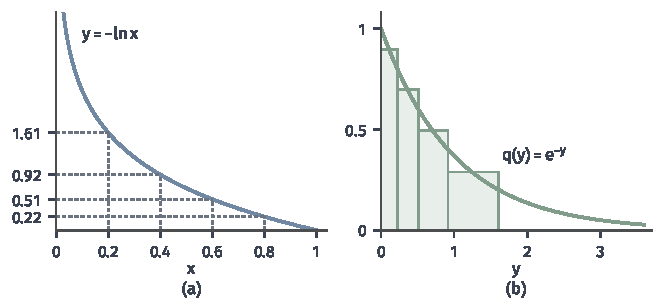
\includegraphics[width=112mm]{figures/04-spaces-measures-and-geometry/02-measure/matplotlib/push-exponential-bins/figure.pdf}
  \caption{由等质量分割看推前密度。(a)映射$y=-\ln x$与$x=0.2,0.4,0.6,0.8$对应的$y$值。(b)绿色矩形的底是长度$0.2$的输入小段映成的区间，面积都是$0.2$，所以高度等于$0.2$除以区间长度；曲线是极限密度$q(y)=\mathrm e^{-y}$。最左的输入小段$(0,0.2]$映到$[1.61,+\infty)$，质量$0.2$落在右侧的尾部，图中未画矩形。}
  \label{fig:push-exponential-bins}
\end{BookInlineFigure}

\subsection{多分支映射}
\label{sec:push-branches}

许多映射不是整体可逆的。$T(x)=x^2$把$x$与$-x$送到同一点，但在$(0,1)$与$(-1,0)$上分别是微分同胚。这类映射的处理办法是把定义域分成几块，在每块上用上一小节的公式，再把落到同一目标点的贡献加起来。

\begin{theorem}[分支映射的推前密度]
\label{thm:push-branch-density}
设$U\subset\mathbb R^d$是开集，$U_1,\ldots,U_m\subset U$是两两不交的开集，例外集$E=U\setminus\bigcup_kU_k$是Lebesgue零测集。设$T:U\to\mathbb R^d$可测，并且每个限制$T_k=T|_{U_k}$是$U_k$到开集$V_k=T(U_k)$的$C^1$微分同胚，$S_k=T_k^{-1}$。若$U$上的测度$\mu$相对于$\lambda_d$有密度$p$，则$T_\#\mu$相对于$\lambda_d$有密度
\begin{equation}
q(\bm y)=\sum_{k=1}^m\mathbf 1_{V_k}(\bm y)\,p\bigl(S_k(\bm y)\bigr)\,\bigl\lvert\det DS_k(\bm y)\bigr\rvert .
\label{eq:push-branch-density}
\end{equation}
\end{theorem}

\begin{proof}
对Borel集$B\subset\mathbb R^d$，把原像按分支拆开，
\[
T^{-1}(B)=\bigl(T^{-1}(B)\cap E\bigr)\cup\bigcup_{k=1}^m\bigl(T^{-1}(B)\cap U_k\bigr),
\]
各部分两两不交。$\mu\ll\lambda_d$，所以$\mu(E)=0$，第一部分不贡献质量。

在第$k$块上，$T^{-1}(B)\cap U_k=T_k^{-1}(B\cap V_k)$。把定理~\ref{thm:push-density-diffeo}用于$T_k$与$U_k$上的测度$\mu|_{U_k}$，其密度是$p$在$U_k$上的限制，得到
\[
\mu\bigl(T_k^{-1}(B\cap V_k)\bigr)=\int_{B\cap V_k}p\bigl(S_k(\bm y)\bigr)\,\lvert\det DS_k(\bm y)\rvert\,\mathrm d\bm y .
\]

对$k$求和，有限个非负积分之和等于和的积分，于是$(T_\#\mu)(B)=\int_Bq\,\mathrm d\lambda_d$。
\end{proof}

定理的三个条件各管一件事。分支两两不交，保证每个原像点只计算一次。例外集$E$是零测集，保证没有遗漏质量；若$T$在一段正长度的区间上取常值，这段不能纳入任何分支，那里可能产生原子，必须另行计算。

各分支的像$V_k$可以重叠。重叠处的点有多个原像，每个原像所在的分支都贡献一项，所以要求和；只取一个逆分支会漏掉其余原像处的质量。可数个分支的情形也成立，此时交换求和与积分的依据是单调收敛定理。

\begin{example}[平方映射]
\label{ex:push-square}
取$[-1,1]$上的均匀概率测度，密度$p=\tfrac12$，$T(x)=x^2$。端点的质量为零，取$U=(-1,1)$。两个分支是$U_1=(0,1)$与$U_2=(-1,0)$，例外集$E=\{0\}$是零测集；两支的像都是$(0,1)$，逆映射分别是
\[
S_1(y)=\sqrt y,\qquad S_2(y)=-\sqrt y ,
\]
导数的绝对值都是$1/(2\sqrt y)$。由式~\eqref{eq:push-branch-density}，在$0<y<1$上
\[
q(y)=\frac12\cdot\frac{1}{2\sqrt y}+\frac12\cdot\frac{1}{2\sqrt y}=\frac{1}{2\sqrt y},
\]
在$(0,1)$外$q=0$。总质量是
\[
\int_0^1\frac{\mathrm dy}{2\sqrt y}=\bigl[\sqrt y\bigr]_0^1=1 .
\]

核对一个集合。取$B=[0.36,0.49]$，原像是$[-0.7,-0.6]\cup[0.6,0.7]$，总长度$0.2$，输入质量是
\[
0.2\times\tfrac12=0.1 .
\]
用输出密度计算，
\[
\int_{0.36}^{0.49}\frac{\mathrm dy}{2\sqrt y}=0.7-0.6=0.1 .
\]
若只取正分支，得到的$1/(4\sqrt y)$总积分只有$\tfrac12$，漏掉了另一半质量。
\end{example}

图~\ref{fig:push-square}左侧显示了例子中的计算：黄色带是输出区间$B$，它在曲线上碰到两个分支，往下落到两段蓝色的输入区间，各贡献质量$0.05$。右侧是相加后的密度，虚线是只取一个分支时的结果。

\begin{BookInlineFigure}
  \centering
  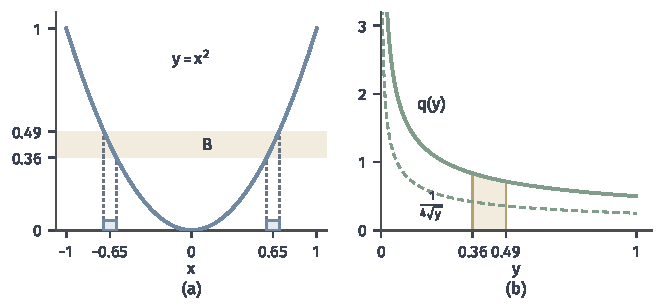
\includegraphics[width=112mm]{figures/04-spaces-measures-and-geometry/02-measure/matplotlib/push-square/figure.pdf}
  \caption{平方映射的推前密度。(a)映射$y=x^2$；输出区间$B=[0.36,0.49]$（黄色带）有两个原像$[-0.7,-0.6]$与$[0.6,0.7]$（蓝色）。(b)实线是两支相加的密度$q(y)=1/(2\sqrt y)$，虚线是只取一个分支的$1/(4\sqrt y)$；$B$上实线下的面积是$0.1$，与输入质量一致。纵轴在$3.2$处截断，$y\to0$时$q$无界但可积。}
  \label{fig:push-square}
\end{BookInlineFigure}

输出密度在$y\to0$时无界，但仍可积。原点的原像只有单点$\{0\}$，输入质量为$0$，所以输出没有点质量。若输入在$0$处有点质量，例如换成$\tfrac12\delta_0+\tfrac14\lambda|_{[-1,1]}$，原测度就不再相对于$\lambda$绝对连续，定理不适用；推前后在$0$处出现点质量$\tfrac12$，这部分不能用相对于长度的密度表示。

\subsection{坐标投影}
\label{sec:push-projection-density}

坐标投影也是多对一映射，但与上一小节不同：落到同一点$x_1$的原像不是有限个点，而是整条\term{纤维}（fiber）$\{x_1\}\times X_2$，其上每一点的质量通常为零。有限分支求和在这里无从谈起，应当沿纤维积分。为此需要原测度相对于乘积参考测度有密度。

\begin{theorem}[边缘密度]
\label{thm:push-marginal-density}
设$(X_1,\mathcal A_1,\mu_1)$与$(X_2,\mathcal A_2,\mu_2)$是$\sigma$有限测度空间，$X_1\times X_2$上的测度$\mu$相对于乘积测度$\mu_1\otimes\mu_2$有密度$p$，$\pi(x_1,x_2)=x_1$。则$\pi_\#\mu$相对于$\mu_1$有密度
\begin{equation}
p_1(x_1)=\int_{X_2}p(x_1,x_2)\,\mu_2(\mathrm dx_2).
\label{eq:push-marginal-density}
\end{equation}
\end{theorem}

\begin{proof}
对$B\in\mathcal A_1$，原像是$\pi^{-1}(B)=B\times X_2$。由密度的定义，再对非负函数用Tonelli定理，
\[
\begin{aligned}
(\pi_\#\mu)(B)&=\mu(B\times X_2)\\
&=\int_{X_1\times X_2}\mathbf 1_B(x_1)\,p(x_1,x_2)\,\mathrm d(\mu_1\otimes\mu_2)\\
&=\int_B\Bigl(\int_{X_2}p(x_1,x_2)\,\mu_2(\mathrm dx_2)\Bigr)\mu_1(\mathrm dx_1).
\end{aligned}
\]
Tonelli定理同时保证内层积分$p_1$是$x_1$的可测函数。于是$(\pi_\#\mu)(B)=\int_Bp_1\,\mathrm d\mu_1$。
\end{proof}

$p_1$取值于$[0,+\infty]$。若$\mu$有限，取$B=X_1$得
\[
\int_{X_1}p_1\,\mathrm d\mu_1=\mu(X_1\times X_2)<+\infty ,
\]
所以$p_1$在$\mu_1$几乎处处有限。

被积函数非负，用Tonelli定理就够了；若要对有符号的$g(x_1)$计算$\int g\,\mathrm d(\pi_\#\mu)$，则要先确认$\int\lvert g\rvert p_1\,\mathrm d\mu_1<+\infty$，这时Fubini定理保证换序。

参考测度取计数测度时，式~\eqref{eq:push-marginal-density}中的积分变成对第二个坐标求和，就是离散联合分布求边缘的公式，也就是图~\ref{fig:push-projection}中逐行逐列的合计。

\begin{example}[正方形上的线性密度]
\label{ex:push-square-marginal}
在$[0,1]^2$上取$\mu$相对于$\lambda_2$的密度$p(x,z)=x+z$。总质量是
\[
\int_0^1\!\!\int_0^1(x+z)\,\mathrm dz\,\mathrm dx=\int_0^1\bigl(x+\tfrac12\bigr)\,\mathrm dx=1 .
\]

第一坐标的边缘密度由式~\eqref{eq:push-marginal-density}算出：
\[
p_1(x)=\int_0^1(x+z)\,\mathrm dz=x+\tfrac12,\qquad0\leq x\leq1 .
\]

核对一个集合。用边缘密度计算，
\[
(\pi_\#\mu)\bigl([0,\tfrac12]\bigr)=\int_0^{1/2}\bigl(x+\tfrac12\bigr)\,\mathrm dx=\tfrac18+\tfrac14=\tfrac38 .
\]
直接用原测度计算，
\[
\mu\bigl([0,\tfrac12]\times[0,1]\bigr)=\int_0^{1/2}\!\!\int_0^1(x+z)\,\mathrm dz\,\mathrm dx=\tfrac38 ,
\]
两者相同。
\end{example}

图~\ref{fig:push-marginal-fiber}把例子中的一条纤维单独取出来。在$x=0.3$处，纤维是竖直的线段，密度沿纤维是$0.3+z$，积分得到$0.3+\tfrac12=0.8$，这就是$p_1(0.3)$。对每个$x$做一次这样的积分，$p_1$的整条曲线就出来了。

\begin{BookInlineFigure}
  \centering
  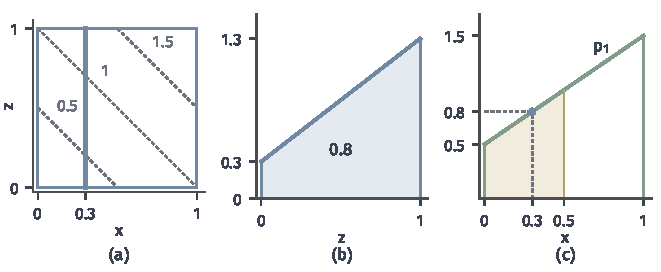
\includegraphics[width=112mm]{figures/04-spaces-measures-and-geometry/02-measure/matplotlib/push-marginal-fiber/figure.pdf}
  \caption{沿纤维积分得到边缘密度。(a)单位正方形上$p(x,z)=x+z$的等值线（虚线，数字是$p$的值），粗线是$x=0.3$处的纤维。(b)沿这条纤维的密度$0.3+z$，阴影面积$0.8$。(c)边缘密度$p_1(x)=x+\tfrac12$，蓝点是(b)算出的值，黄色面积是$[0,\tfrac12]$上的质量$\tfrac38$。}
  \label{fig:push-marginal-fiber}
\end{BookInlineFigure}

\paragraph{与分支求和的区别}
投影与分支映射都是多对一的，但累计方式不同。分支映射的每个目标点只有有限个原像，每个原像附近映射是局部微分同胚，贡献由Jacobian因子换算后相加。投影的原像是整条纤维，纤维上单点没有质量，贡献必须用纤维上的参考测度$\mu_2$积分。表~\ref{tab:push-mechanisms}汇总了本节的三种机制。

\begin{BookInlineTable}
  \centering
  \begin{tabular}{@{}llll@{}}
    \toprule
    & 微分同胚 & 多分支映射 & 坐标投影\\
    \midrule
    目标点的原像 & 一个点 & 有限个点 & 一条纤维\\
    参考测度 & Lebesgue测度 & Lebesgue测度 & 乘积测度\\
    密度的来源 & 逆映射Jacobian & 各分支相加 & 沿纤维积分\\
    依据 & 经典换元公式 & 逐分支换元 & Tonelli定理\\
    \bottomrule
  \end{tabular}
  \caption{三种计算推前密度的机制。}
  \label{tab:push-mechanisms}
\end{BookInlineTable}

累次积分的依据是乘积结构：$\mu$的参考测度是乘积测度，纤维恰好是坐标截面。一般的非线性降维没有现成的乘积结构，必须另行核对沿纤维积分的条件，以及纤维上用什么参考测度。一种可行的做法是先用微分同胚把纤维拉直成坐标截面，再投影。

以单位圆盘$D$上的均匀概率测度为例，密度是$1/\pi$，映射$R(x,z)=\sqrt{x^2+z^2}$把点送到它到原点的距离，纤维是同心圆周。为把圆周拉直，先去掉零测的射线$\{(x,0):x\geq0\}$，此后极坐标
\[
\Phi(r,\theta)=(r\cos\theta,r\sin\theta)
\]
是$G=(0,1)\times(0,2\pi)$到圆盘剩余部分的微分同胚，Jacobian行列式是$r$。

令$T=\Phi^{-1}$，由式~\eqref{eq:push-density-diffeo}，$T_\#\mu$相对于$G$上面积的密度是
\[
q(r,\theta)=\frac1\pi\cdot r=\frac r\pi .
\]
$R$就是$T$与第一坐标投影$\pi_1$的复合，由复合规则~\eqref{eq:push-composition}和定理~\ref{thm:push-marginal-density}，半径的密度是
\[
p_R(r)=\int_0^{2\pi}\frac r\pi\,\mathrm d\theta=2r,\qquad0<r<1 .
\]

核对一个集合：半径不超过$s$的质量是面积比$s^2$，而$\int_0^s2r\,\mathrm dr=s^2$。图~\ref{fig:push-polar-fibers}中的黄色环带取$0.5<r\leq0.6$，三幅图里的质量都是$0.6^2-0.5^2=0.11$。

\begin{BookInlineFigure}
  \centering
  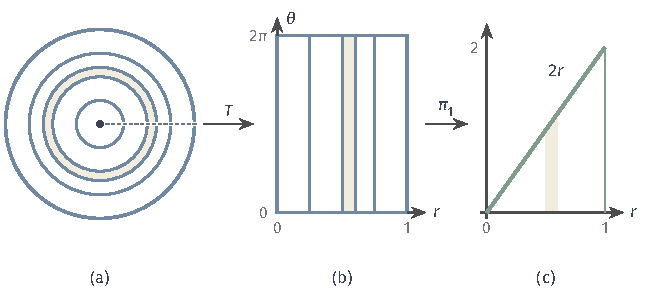
\includegraphics[width=109.813mm]{figures/04-spaces-measures-and-geometry/02-measure/tikz/push-polar-fibers/figure.pdf}
  \caption{先把纤维拉直再投影。(a)单位圆盘上$R(x,z)=\sqrt{x^2+z^2}$的几条纤维（同心圆周），虚线是去掉的射线。(b)极坐标平面上，同一批纤维变成竖直线段。(c)对$\theta$积分后得到半径的密度$2r$。黄色部分是$0.5<r\leq0.6$的同一批点，质量都是$0.11$。}
  \label{fig:push-polar-fibers}
\end{BookInlineFigure}

这个例子说明纤维上的参考测度不能想当然。直接对$\theta$积分平面密度$1/\pi$，得到常数$2$，总质量变成$2$，这是漏掉了Jacobian因子$r$。沿圆周用弧长积分$1/\pi$，得到$2\pi r/\pi=2r$，结果正确；但这个正确是有条件的。

换一个输出函数$t=x^2+z^2$，纤维还是同样的圆周。由半径的密度$2r$和映射$r\mapsto r^2$，用式~\eqref{eq:push-density-diffeo}，$t$的密度是
\[
2\sqrt t\cdot\frac{1}{2\sqrt t}=1,\qquad0<t<1 .
\]
这时沿圆周用弧长积分$1/\pi$仍然得到$2\sqrt t$，它在$(0,1)$上的总积分是$\tfrac43$，并不是$1$。

差别来自相邻两条纤维之间的距离。半径增加$\mathrm dr$时，相邻圆周的间距恰好是$\mathrm dr$；$t$增加$\mathrm dt$时，间距是$\mathrm dt/(2\sqrt t)$，所以弧长积分还要乘这个因子。同一族纤维，输出函数不同，纤维上应当使用的权重也不同，这就是一般降维必须单独核对的内容。

\section{本章小结}
\label{sec:push-summary}

本章开头问：原空间上的质量经可测映射后怎样分布在目标空间上，目标空间上的积分怎样回到原空间计算。第一个问题由原像回答。推前测度$T_\#\mu(B)=\mu(T^{-1}(B))$把目标集合的质量规定为它的原像的质量；原像保持不交并，所以推前测度可数可加，总质量不变，并且分步推前与一次推前相同。$\sigma$有限性则可能在推前时丢失，用到相关定理时要单独核对。

例子显示了推前测度记录什么、丢掉什么。一一映射只搬动质量；多对一映射在同一输出点汇合质量，丢掉原像之间的区分，甚至把区间上的长度汇合成点质量；伸缩改变长度的比例；坐标投影只保留柱形集合上的值，两个边缘合起来也不能恢复联合测度。

第二个问题由推前积分恒等式$\int_Yg\,\mathrm d(T_\#\mu)=\int_Xg\circ T\,\mathrm d\mu$回答。它沿积分的构造从指示函数推广到非负函数，再在绝对可积条件下推广到有符号与复值函数。恒等式只用到原像，不要求映射可逆，也不要求任何密度；它与上一章的换测度公式不同，后者点不移动，只改变累计权重。

在目标空间选定参考测度后，两步改写把原空间的积分化为目标空间的加权积分，前提是推前测度有密度；常值映射把正长度的区间压成一点，说明这个前提可以失败。

三种计算机制各有依据，不能互相替代。微分同胚的推前密度是$p(T^{-1}(\bm y))\lvert\det DT^{-1}(\bm y)\rvert$，因子在新坐标上取值、方向是逆映射，它与通常换元公式中在原坐标上取值的正向Jacobian互为对照，伸缩映射可以核对方向。多分支映射要求分支不交、例外集零测，再对落到同一点的有限个原像分支求和。坐标投影的原像是整条纤维，需要乘积参考测度，用Tonelli定理沿舍去的坐标积分；一般的非线性降维还要另行确定纤维上的参考测度，例如先用极坐标把纤维拉直再投影。

这些结论完成了测度部分的主线：从集合的测量到函数的积分，从同一空间上的换测度到空间之间的推前。第三部分将在这些积分工具之上研究函数空间的范数、完备性与逼近；流形上的体积测度与积分，即本章坐标换元在弯曲空间上的推广，在第~\ref{chap:manifold-calculus}章研究。

